\documentclass[12pt,a4paper]{scrartcl} 

%Deutsch:
	\usepackage[ngerman]{babel} %Deutsches Datumformat, Umlaute m\"oglich,...
	\usepackage[utf8]{inputenc}
	\usepackage[T1]{fontenc} 
	
%Quellenverzeichnis:
	\usepackage[maxcitenames=2,autocite=footnote,uniquename=full,uniquelist=true,backend=biber]{biblatex} %style=authoryear-icomp
	\usepackage{csquotes} %Hilfspaket für Biblatex
	\bibliography{bib_database.bib} %Datei mit bibliographischen Daten
	\DefineBibliographyStrings{ngerman}{andothers={et\ al\adddot}} % "u.a." zu "et al."
	\DefineBibliographyStrings{ngerman}{and={\&}} % "und" zu "&"

%Mathematik:
	\usepackage{dsfont} %Symbole
	\usepackage{amsmath} %Umgebung
	\usepackage{amssymb} %Symbole
	\usepackage{bbm} %doppelstreifen bei buchstaben (zb symbol für ganze zahlen \mathbbm{Z})
	
%Grafiken:
	\usepackage{graphics}
	\usepackage{graphicx}
	\usepackage{picinpar} %bilder so einfügen, dass text um bilder weiterläuft
	\usepackage{float} %\begin{figure}[H] => Grafik wird HIER eingefügt!

%Euro-Zeichen:
	\usepackage{eurosym}

%Pseudo Code:
	\usepackage{algorithmic}
	\usepackage{algorithm}
	\renewcommand{\algorithmicrequire}{\textbf{Eingabe:}}
	\renewcommand{\algorithmicensure}{\textbf{Ausgabe:}}

%Verzeichnis-struktur darstellen:
	\usepackage{dirtree}

%Tabellen:
	\usepackage{multirow}
	
%Quellcode:
	%\usepackage[numbered,framed]{mcode} %Quellcode darstellen
	
%Englisch:
	%\usepackage[ngerman,english]{babel} %automatisch erzeugte Überschriften etc. auf englisch
	
\DeclareMathOperator*{\argmin}{arg\,min} % Importiere die Einstellungen aus der Präambel

%%%%%%%%%%%%%%%%%%%%%%%%%%%%%%%%%%%%%%%%%%%%%%%%%%%%%%%%%%
% Hier können die Pakete, die benötigten Daten und Graphen für R geladen bzw erstellt werden.
% echo=FALSE gibt keinen R Output wieder
% warum wird der folgende chunk nicht übernommen?



% hier beginnt der eigentliche Inhalt
\usepackage{Sweave}
\begin{document}
\input{Bericht_Sweave-concordance}

% Deckblatt
\begin{titlepage}
	\rmfamily
	\begin{center}
		% Logo
		%\includegraphics[width=0.15\textwidth]{./logo}\\[1cm]
	
		\textsc{\LARGE Statistisches Consulting}\\[1.5cm]

		\textsc{
			\large{	Master Studiengang Statistik\\[0.25cm]
							Institut für Statistik\\[0.25cm]
							Ludwig-Maximilians-Universität München}}\\[0.25cm]
						
		% Title
		\newcommand{\HRule}{\rule{\linewidth}{0.5mm}}
		\HRule \\[0.4cm]
		{\huge \bfseries Online-Marketing der Interhyp AG\\[0.5cm]Analyse von Tracking-Daten}\\[0.4cm]
		\HRule \\[1.5cm]
		
		% Autoren
		\textbf{Daniel Fuckner} d.fuckner@gmx.de\\
		\textbf{Markus Vogler} markus@vogler-lindau.de\\[1.5cm]
	
		% Betreuer und Projektpartner
		\begin{minipage}{0.4\textwidth}
			\begin{flushleft}
				Projektpartner:\\
				\textbf{Nicola Gries} (Interhyp AG)
			\end{flushleft}
		\end{minipage}
		\hfill
		\begin{minipage}{0.4\textwidth}
			\begin{flushright}
				Betreuer:\\
				\textbf{Dr. Fabian Scheipl}
			\end{flushright}
		\end{minipage}
		
		\vfill

		% Datum
		{\large München, 26.08.2014}
		
	\end{center}
\end{titlepage}

%\thispagestyle{plain}
\pagenumbering{roman} %römische Seitennummerierung

%Abstract
\begin{abstract}
  \noindent
	\paragraph{Abstract:}
	\paragraph{Background:} In patients with
\end{abstract}

%Inhaltsverzeichnis
\newpage
\tableofcontents

\newpage
\pagenumbering{arabic} %ab hier wieder normale Seitennummerierung

% Hier beginnt der eigentliche Text
\section{Einleitung} 

\begin{frame}\frametitle{Einleitung} 
	\begin{itemize}
		\item Interhyp AG ist Vermittler für private Baufinanzierungen
		\item Primäres Ziel des Marketing ist die Kundenakquise
		\item Etwa $80 \%$ aller Kundenanträge werden online abgeschickt
		\item Online-Marketing verfügt über verschiedene Kanäle
		\item Refined Labs GmbH ist verantwortlich für das Online-Tracking der Werbekampagnen der Interhyp AG
	\end{itemize}
\end{frame}

\begin{frame}\frametitle{Entstehung eines Funnels (Quelle: Interhyp AG)}
	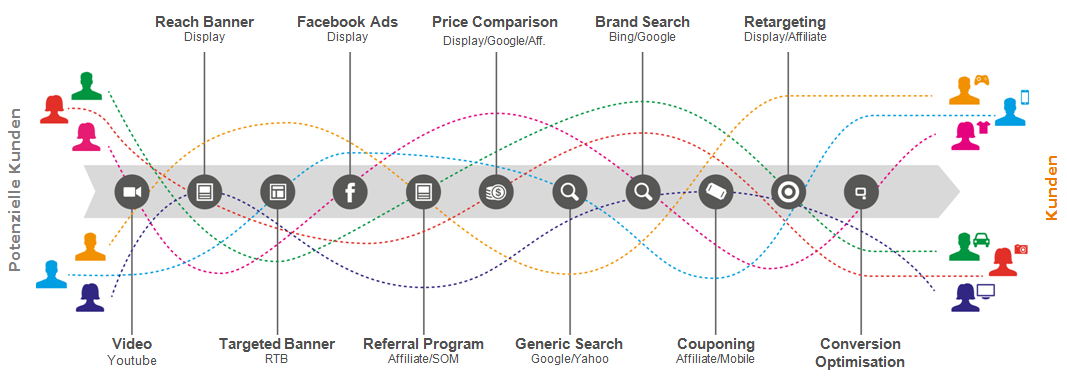
\includegraphics[scale=0.38]{customerJourney.png}\\
	\centering Unterschiede zwischen konvertierten und nicht-konvertierten Funnels?
\end{frame} % Importiere die Einleitung
\section{Datenlage}\label{datenlage}

Die Daten wurden von der Refined Labs GmbH als SQL-Dump bereitgestellt, der eine Größe von circa $13$ Gigabyte hat. Die MySQL-Datenbank enthält die vier Tabellen \textit{project\_out}, \textit{redirects\_short}, \textit{searchFunnel} und \textit{stage2\_transactionHandling}. Mit Hilfe der vorhanden Informationen in \textit{searchFunnel} und \textit{stage2\_transactionHandling} konnten die Kontaktpunkte in \textit{redirects\_short} in konvertierte und nicht-konvertierte Funnels unterteilt werden. In \textit{projects\_out} sind die Kampagnen in Form einer Baumstruktur organisiert. In Absprache mit der Interhyp AG wurden $17$ Kategorien ausgewählt, die sich auf den ersten drei Ebenen dieser Baumstruktur befinden. Anhand von IDs wurde jedem Kontaktpunkt eine dieser Kategorien zugewiesen.\\
Tabelle \ref{exdata} enthält ein Datenbeispiel mit den Spalten \textit{ID}, \textit{Campaign}, \textit{Transaction} und \textit{Position}. Das Beispiel enthält zwei verschiedene \textit{IDs}, das heißt zwei Funnels, wobei der erste vier und der zweite drei Kontaktpunkte hat. Die Spalte \textit{Campaign} enthält die Kampagne der Kontaktpunkte. \textit{Transaction} ist eine binäre Variable und gibt an, ob der Kunde konvertiert ist, wobei der Wert $1$ nur für den letzten Kontaktpunkt vor der Konvertiertung angenommen wird. Das heißt bei \textit{ID} $1$ handelt es sich um einen konvertierten und bei \textit{ID} $2$ um einen nicht-konvertierten Funnel. Die \textit{Position} gibt die Nummer des Kontaktpunktes an und reicht damit von $1$ bis zur Länge des Funnels.\\
\begin{table}[H]
	\begin{center}
		\begin{tabular}{|c|l|c|c|c|c|}
			\hline
			ID & Campaign 									 & Transaction & Position & ... \\ \hline\hline
			1  & Affiliate - Partnerprogramm & 0					 & 1		    & ... \\ \hline
			1  & SEM - Brand                 & 0					 & 2		    & ... \\ \hline
			1  & Direct                      & 0					 & 3		    & ... \\ \hline
			1  & Direct                      & 1					 & 4		    & ... \\ \hline
			2  & Display                     & 0					 & 1		    & ... \\ \hline
			2  & SEM - Generisch             & 0					 & 2		    & ... \\ \hline
			2  & Social Media                & 0					 & 3		    & ... \\ \hline
		\end{tabular} 
	\end{center}
	\caption{Beispiel für einen Auszug aus der Datenbank}\label{exdata}
\end{table}
Nun sollen noch die verschiedenen Kategorien des Features \textit{campagin}, das heißt die verschiedenen Werbeformen betrachtet werden. Tabelle \ref{beschreibungCampaign} enthält Erklärungen der $17$ verwendeten Kategorien.\\
\textit{Affiliate - Partnerprogramm} sind Partner, die von der Interhyp AG bereitgestellte Werbemittel wie Rechner, Logo oder Banner einbinden. Partner, die einen Zinsvergleich bereitstellen, welcher das Zinsangebot der Interhyp AG mit deren Wettbewerbern im Vergleich dargestellt, gehören \textit{Affiliate - Rest} an. \textit{Direct} bedeutet, dass ein potentieller Kunde im Browser direkt \textit{www.interhyp.de} eingibt und \textit{Display} sind Bannerschaltungen auf diversen Webseiten. \textit{E-Mailing} umfasst Mails an Interessenten, die bereits einen Antrag gestellt oder ein Infopaket angefordert haben. Wenn ein potentieller Kunde über einen unbezahlten Link zur Interhyp AG gelangt, so wird der Kontaktpunkt der Kampagne \textit{Generic} zugewiesen. \textit{Kooperationen} sind individuelle Zusammenarbeiten mit größeren Partnern, die je nach Vertrag verschiedene Werbemittel auf ihrer Seite einbinden und \textit{Newsletter} sind regelmäßige Rundschreiben. \textit{SEM} sind bezahlte Suchergebnisse, wobei \textit{Brand} bedeutet, dass die Suchanfrage das Wort \textit{Interhyp} beinhaltete, \textit{Generisch} bedeutet, dass etwas wie \textit{Baufinanzierung} oder ähnliches gesucht wurde und \textit{Remarketing} bedeutet, dass der potentielle Kunde bereits zuvor auf der Seite der Interhyp AG war und deshalb erneut eine Werbeeinblendung der geschaltet wurde. Unbezahlte Suchergebnisse werden \textit{SEO} zugewiesen und \textit{Social Media} umfasst Werbung auf \textit{Facebook} und \textit{gutefrage.net}.
\begin{table}[H]
	\begin{center}
		\begin{tabular}{|l|p{9cm}|}
			\hline \textbf{Kampagne} & \textbf{Beschreibung}\\ \hline
			\hline Affiliate - Partnerprogramm & Partner, die Werbemittel einbinden\\
			\hline Affiliate - Rest & Partner, die Zinsvergleich bereitstellen\\ 
			\hline Direct & Direkte Eingabe von \textit{www.interhyp.de}\\ 
			\hline Display & Bannerschaltungen\\
			\hline E-Mailing & Mails an Interessenten, die schon einen Antrag o.ä. gestellt haben\\
			\hline Generic & Unbezahlter Link\\
			\hline Kooperationen - Focus & \multirow{5}{6cm}{Individuelle Zusammenarbeit mit größeren Partnern}\\
			Kooperationen - Immonet & \\
			Kooperationen - Immoscout24 & \\
			Kooperationen - Immowelt & \\
			Kooperationen - Rest & \\
			\hline Newsletter & Regelmäßige Rundschreiben\\
			\hline SEM - Brand & \multirow{3}{6cm}{Bezahlte Suchergebnisse}\\
			SEM - Remarketing & \\
			SEM - Generisch & \\
			\hline SEO & Unbezahlte Suchergebnisse\\
			\hline Social Media & \textit{facebook} und \textit{gutefrage.net}\\
			\hline
		\end{tabular} 
	\end{center}
	\caption{Beschreibung der Kampagnen}\label{beschreibungCampaign}
\end{table}
Ein Kontaktpunkt mit einer der $17$ Kampagnen tritt entweder in der Form eines \textit{Clicks} oder eines \textit{Views} auf. Man spricht von einem \textit{Click}, wenn der potentielle Kunde tatsächlich etwas angeklickt hat und ein \textit{View} wird getrackt, wenn ein Banner oder ähnliches lediglich gesehen, aber nicht angeklickt wird. An dieser Stelle wirft die Datenerhebung allerdings ein Problem für die statistischen Analysen auf. Die \textit{Views} werden für alle konvertierten Funnels gespeichert, für die nicht-konvertierten Funnels allerdings nur, wenn diese bei einem anderen Kunden der Refined Labs GmbH konvertieren. Dass heißt, es ist eine systematische Veränderung der Daten gegeben. Deshalb besteht keine Möglichkeit die \textit{Views} in statistische Analysen, die konvertierte und nicht-konvertierte Funnels vergleichen, einzubeziehen. Die \textit{Views} werden lediglich in Kapitel \ref{descriptiv} in einigen Plots betrachtet, die nur konvertierte Funnels enthalten, und von den weiteren Analysen ausgeschlossen.\\
Nach der Vorverarbeitung der Daten, die mit \textit{MySQL 6.1} und \textit{R 3.0.2} \cite{r} durchgeführt wurde, liegen $ 297,963 $ \textit{Clicks} für die konvertierten und $ 9,550,802 $ \textit{Clicks} für die nicht-konvertierten Funnels vor. Zum Handhaben der großen Datenmenge wurden die Pakete \textit{data.table} \cite{data.table} und \textit{plyr} \cite{plyr} verwendet. Eine nähere Beschreibung der in \textit{R} erstellten Features erfolgt in Kapitel \ref{descriptiv}.\\




\section{Zeitdiskretes Survival-Modell}\label{survival}

\subsection{Lebensdauer-Modell}\label{secModel1}

Aufgrund der in Kapitel \ref{datenlage} beschriebenen Datenlage erscheint die Anwendung eines Modells aus dem Feld der Lebensdaueranalyse intuitiv. Es wird die Zeit bis zu einem Ereignis betrachtet, welches in diesem Fall das Ausfüllen eines Online-Antrages ist. Der potentielle Kunde befindet sich während der Beobachtungsspanne im transienten Zustand bis er durch die Konvertierung in den absorbierenden Zustand wechselt, an dem die Beobachtung endet. Tritt am Ende der Beobachtung keine Konvertierung ein, so spricht man von einer Rechtszensierung.\\
Die Position gibt die Nummer des Kontaktpunktes an und bildet die Zeitachse des Modells. Das heißt, es handelt sich um ein zeitdiskretes Modell und die Zielvariable $y_{ip}$ (\ref{zielvar}) nimmt den Wert Eins an, wenn Kunde $i$ an der Position $p$ konvertiert ist. Für alle vorherigen Positionen eines konvertierten Funnels und für alle Positionen eines nicht-konvertierten Funnels nimmt $y_{ip}$ den Wert Null an. $N_p$ ist die Anzahl der Beobachtungen an Position $p$. Diese nimmt mit steigendem $p$ ab, da in jeder Position Funnels konvertieren oder Beobachtungen ohne Konvertierung enden. Deshalb wird das Modell nur auf die ersten $25$ Positionen angewendet, da für spätere Positionen nicht ausreichend konvertierte Funnels vorliegen.\\
\begin{align}
	y_{ip} = \begin{cases} 1 & \text{Beobachtung } i \text{ konvertiert an Position } p\\
												 0 & \text{sonst} 
					 \end{cases} \text{, } p=1,...,25 \text{, } i=1,...,N_p \label{zielvar}
\end{align}
Das Modell schätzt die Hazardrate $\lambda_{ip}$ (\ref{haz}), das heißt die Wahrscheinlichkeit, dass Beobachtung $i$ an Position $p$ konvertiert unter der Bedingung, dass die Länge des Funnels von Beobachtung $i$ größer oder gleich $p$ ist, was lediglich bedeutet, dass für Beobachtung $i$ an Position $p$ überhaupt noch ein Kontaktpunkt vorliegt. Außerdem wird auf die Features $x_{ip}$ bedingt, die später noch näher erläutert werden.
\begin{align}
	\lambda_{ip} = P(y_{ip}=1|funnelLength_i \geq p, x_{ip}) \label{haz}
\end{align}
Die Hazardrate wird mittels eines Logit-Modells (\ref{logit1}-\ref{logit2}) mit der Zielvariable $y_{ip}$ an jeder Position $p$ seperat geschätzt. Die Annahmen des Modells sind, dass die $y_{ip}|x_{ip}$ unabhängig Bernoulli-verteilt sind mit der Hazardrate $\lambda_{ip}$ als Parameter und der Erwartungswert wird anhand der Responsefunktion $h$ mit der Prädiktorfunktion $f_{p}$ verknüpft.
\begin{align}
	y_{ip}|x_{ip} &\stackrel{ind}{\sim} Bin(1, \lambda_{ip}) \label{logit1} \\
	E(y_{ip}|x_{ip}) = P(y_{ip} = 1|x_{ip}) = \lambda_{ip} &= h(f_{p}(x_{ip})) = \frac{\exp(f_{p}(x_{ip}))}{1+\exp(f_{p}(x_{ip}))}\label{logit2}
\end{align}
Aus diesen Annahmen lassen sich Likelihood (\ref{lik}) und Log-Likelihood (\ref{loglik}) des Modells ableiten.
\begin{align}
	L(\lambda_{ip}) &= \prod_{i=1}^{N_p} \lambda_{ip}^{y_{ip}} (1-\lambda_{ip})^{1-y_{ip}} \label{lik} \\
	l(\lambda_{ip}) &= \ln(L(\lambda_{ip})) = \sum_{i=1}^{N_p} (y_{ip} \ln(\lambda_{ip}) + (1-y_{ip}) \ln(1-\lambda_{ip})) \notag \\
	&= \sum_{i=1}^{N_p} (y_{ip} f_p(x_{ip}) - \ln(1+\exp(f_p(x_{ip})))) \label{loglik}
\end{align}
Damit ergibt sich der binomielle Verlust aus der negativen Log-Likelihood (\ref{binVer}) und das Logit-Modell ist lösbar durch die Minimierung dieses Verlusts.
\begin{align}
	L(y_{ip},f_p(x_{ip})) = -\sum_{i=1}^{N_p} (y_{ip} f_p(x_{ip}) + \ln(1+\exp(f_p(x_{ip}))))
\end{align}
Um ein gutes Prognose-Modell zu entwickeln, wird eine Ensemble-Methode angewendet, die im nächsten Abschnitt vorgestellt wird.

\subsection{Stochastic Gradient Boosting}\label{secModel2}

\subsubsection*{Algorithmus}

Stochastic Gradient Boosting ist eine Ensemble-Methoden, die durch mehrfache Anwendung des sogenannten Basis-Lerners ein Ensemble von Schätzern für eine Prognosefunktion liefert. Durch Aggregation der Schätzer erhält man die endgültige Prognosefunktion. Ein sehr beliebter Basis-Lerner sind Stümpfe, das heißt Bäume mit nur einem Split. Einige Vorteile von Bäumen sind, dass sie mit kategoriellen Features, Ausreißern und fehlenden Werten umgehen können. Außerdem wird der schwachen Prognoseleistung von Bäumen durch die Kombination mit Boosting entgegen gewirkt.\\
Gesucht ist also eine Prognosefunktion, die den Erwartungswert einer Verlustfunktion minimiert. Als Verlustfunktion wird der binomielle Verlust (\ref{binVer}) verwendet, wobei sich die Prädiktorfunktion wie folgt ergibt.
\begin{align}
	f(x_{ip}) =& \text{offset}(\hat{\lambda}_{i,p-1}) + \notag \\
						 &f_{weekday,p}(\text{weekday}_{ip}) + \notag \\
						 &f_{hour,p}(\text{hour}_{ip}) + \notag \\
						 &f_{campaign,p}(\text{campaign}_{ip}) + \notag \\
						 &f_{campaignLast,p}(\text{campaign}_{i,p-1}) + \notag \\
						 &f_{campaignLast2,p}(\text{campaign}_{i,p-2}) + \notag \\
						 &f_{timeSinceLast,p}(\text{timeSinceLast}_{ip}) + \notag \\
						 &f_{timeSinceFirst,p}(\text{timeSinceFirst}_{ip}) \label{praediktor}
\end{align}
Der Prädiktor ist also eine additive Funktion von Treppenfunktionen der sieben verwendeten Features und einem offset. Hier sei nochmal darauf hingewiesen, dass Features wie \textit{hasClicked} oder \textit{clickCount} nicht verwendet werden können, da die Views aufgrund der Problematik der Datenerhebung nicht berücksichtigt werden. Die verwendeten Einflussgrößen sind also der Wochentag und die Stunde des jeweiligen Kontaktpunktes, die Kampagne des aktuellen und der letzten zwei Kontakte, sowie die Dauer seit dem vorherigen Kontaktpunkt und die Gesamtdauer seit dem ersten bis zum jetzigen Kontakt. Die Funktionen $f_{.,p}$ können theoretisch für verschiedene Positionen komplett unterschiedliche Formen annehmen. Es sei ausdrücklich darauf hingewiesen, dass $f_{campaignLast,p}(\textit{campaign}_{i,p-1})$ und $f_{campaign,p-1}(\textit{campaign}_{i,p-1})$ zwei unterschiedliche Funktionen sind. Erstere gibt den Einfluss der Art des vorherigen Kontaktpunktes auf die Konvertierungswahrscheinlichkeit an der Position $p$ wieder und zweitere den Einfluss der Art des aktuellen Kontaktpunktes auf die Konvertierungswahrscheinlichkeit an der Position $p-1$. Unter der Annahme, dass der Einfluss der Features an den verschiedenen Positionen ähnlich ist, fließt zusätzlich noch die Vorhersage des Modells der vorherigen Position als offset mit ein. Dadurch konnten die Ergebnisse besonders an späteren Positionen, an denen weniger Daten vorhanden sind, deutlich verbessert werden. Ergebnisse ohne offset sind im elektronischen Anhang zu finden.\\
Der offset fällt für Position eins weg, da es noch keine Vorhersagen eines vorherigen Modells gibt. Außerdem sind für Position eins die Features \textit{campaignLast}, \textit{campaignLast2}, \textit{timeSinceLast} und \textit{timeSinceFirst} offentsichtlich noch nicht vorhanden, so dass diese ebenfalls wegfallen. An Position zwei ist \textit{campaignLast2} noch nicht vorhanden und \textit{timeSinceLast} und \textit{timeSinceFirst} sind hier identisch, so dass nur eine der beiden berücksichtigt wird. Ab Position Drei ergibt sich der Prädiktor dann exakt so wie in (\ref{praediktor}) dargestellt.\\
\floatname{algorithm}{Algorithmus}
\begin{algorithm}
\caption{Gradient Boosting}\label{alg}
\label{gradboosting}
\begin{algorithmic}
\STATE Setze Startwert für $f_{0p}(x_{ip})$
\FOR{$m=1:n.trees$}
	\STATE Setze $\lambda_{ip}(x_{ip}) = \frac{\exp(f_{m-1,p}(x_{ip}))}{1+\exp(f_{m-1,p}(x_{ip}))}$
	\FOR{$i=1:N_p$} 
		\STATE $r_{imp} = - \frac{\partial L(y_{ip},f_{m-1,p}(x_{ip}))}{\partial f_{m-1,p}(x_{ip})} = y_{ip} - \lambda_{ip}(x_{ip})$
	\ENDFOR
	%\STATE Fit a regression base learner to the pseudo-residuals $r_{im}$:
	\STATE Fitte Stumpf: $\theta_{mp} = \argmin_{\theta} \sum_{i=1}^{N_p} (r_{imp} - h(x_{ip}, \theta))^2$
	\STATE Line-Search: $\beta_{mp} = \argmin_{\beta} \sum_{i=1}^{N_p} L(y_{ip}, f_{m-1,p}(x_{ip}) + \beta h(x_{ip},\theta_{mp}))$
	\STATE Update: $f_{mp}(x_{ip}) = f_{m-1,p}(x_{ip}) + \beta_{mp} h(x_{ip},\theta_{mp})$
\ENDFOR
\end{algorithmic}
\end{algorithm}
Algorithmus \ref{alg} enthält Pseudo-Code, der das grobe Vorgehen beim Gradient Boosting erläutern soll. Dieser muss für jedes $p=1,...,25$ durchgeführt werden. Zunächst muss ein Startwert des Prädiktors an Position $p$ festgelegt werden. Daraufhin werden folgende Schritte für $m=1$ bis \textit{n.trees} iteriert. Zunächst werden die Hazardraten $\lambda_{ip}$ durch Rücktransformation der Prädiktorfunktion aus der vorherigen Iteration berechnet. Für jede Beobachtung $i$ werden dann die Pseudo-Residuen $r_{imp}$ berechnet, die die Richtung des negativen Gradienten angeben. Die Pseudo-Residuen entsprechen also der Richtung des steilsten Abstiegs der Verlustfunktion. An die Pseudo-Residuen wird ein Basis-Lerner $h(x_{ip},\theta_{mp})$, in diesem Fall ein Entscheidungsbaum, so angepasst, dass er den negativen Gradienten so gut wie möglich approximiert. Bildlich gesprochen wird das Modell also in die Richtung der größten Verringerung des Verlusts verschoben. Da als Basis-Lerner Stümpfe verwendet werden, wird die Verbesserung des Modells in einem Boosting-Schritt durch nur eines der sieben Features erklärt. Per Line-Search wird daraufhin die optimale Schrittweite $\beta_{mp}$ berechnet und das Modell wird geupdatet mit $f_{mp}(x_{ip}) = f_{m-1,p}(x_{ip}) + \beta_{mp} h(x_{ip},\theta_{mp})$. Nach \textit{n.trees} Iterationen endet der Algorithmus.\\
Durch die Verringerung des Verlusts in jeder Iteration kann es vor allem bei einer hohen Anzahl von Iterationen zu Overfitting kommen. Deshalb wird mittels Kreuzvalidierung die optimale Anzahl an Iterationen ausgewählt. Das heißt $\hat{f}(x_{ip}) = f_{m\_opt,p}(x_{ip})$ wird als Ergebnis verwendet. Das Ensemble der Splits bis zur optimalen Iterationsanzahl bildet für jedes der Feautures eine Treppenfunktion.

\subsubsection*{Parameter des Modells}

Das Modell wurde mit dem Paket \textit{gbm} \cite{gbm} berechnet und mit Hilfe der R-Pakete \textit{foreach} \cite{foreach} und \textit{doSNOW} \cite{dosnow} parallelisiert. Die Modelle für die einzelnen Positionen können allerdings nur dann parallelisiert werden, wenn kein offset benützt wird. Für die Anwendung des Modells müssen noch einige Parameter eingestellt werden.\\
Zunächst wurden die Daten in Trainings- und Testdaten aufgeteilt, sodass Trainings- und Testdaten jeweils die Hälfte der gesamten Daten ausmachen. Da die Anzahl der nicht-konvertierten Funnels deutlich überwiegt und einige Kampagnen vergleichsweise selten in den Daten auftreten, wurden die Trainingsdaten stratifiziert bezüglich konvertierter beziehungsweise nicht-konvertierter Funnel und der Variable \textit{Campaign} gezogen. Außerdem wurde die Länge der Funnels bei der Ziehung berücksichtigt, so dass  Trainings- und Testdaten positionsübergreifend klar getrennt sind und das Verhältnis von eins zu eins trotzdem eingehalten wird. Das heißt, dass eine Beobachtung, die an Position $1$ in den Trainingsdaten enthalten ist auch an allen späteren Positionen in den Trainingsdaten ist. Das selbe gilt für die Testdaten. Dies ist wichtig, damit Trainings- und Testdaten bei der Anwendung des offsets nicht vermischt werden. Anhand der Trainingsdaten wurde das Modell gefittet. Die Testdaten dienen der späteren Bewertung der Prognosegüte des Modells.\\
Die maximale Anzahl der Bäume \textit{n.trees} wurde gleich $3000$ gesetzt, wobei für die Präsentation der Ergebnisse die optimale Anzahl an Bäumen mittels 5-facher Kreuzvalidierung gewählt wurde. Dafür werden die Trainingsdaten in fünf gleich große Partitionen aufgeteilt. Dann wird der Gradient Boosting-Algorithmus fünf mal angewendet, wobei jeweils eine Partition der Daten außen vorgelassen wird. Anhand dieser Partition wird dann der binomielle Verlust nach jeder Iteration mit der aktuellen Prognosefunktion berechnet. Das führt für jede Iteration zu fünf Schätzern für den binomiellen Verlust. Diese fünf Schätzer werden für jede Iteration gemittelt und die Iteration mit dem geringsten binomiellen Verlust wird als optimale Iterationsanzahl gewählt. Daraufhin wird der Gradient Boosting-Algorithmus auf alle fünf Partitionen angewendet.\\
Zusätzlich zu der Beschränkung der Iterationen, wird dem Overfitting auch durch einen Shrinkage-Parameter $\mu$ entgegen gewirkt. Dieser bewirkt, dass nicht die optimale Schrittweite $\beta_{mp}$ in jeder Iteration gegangen wird, sondern nur ein Bruchteil dieser Schrittweite. Es wird also durch $f_{mp}(x_{ip}) = f_{m-1,p}(x_{ip}) + \mu \beta_{mp} h(x_{ip},\theta_{mp})$ geupdatet, wobei $\mu$ gleich $0.01$ gewählt wurde, was einem üblichen Wert für diesen Parameter entspricht. Bei der Wahl von $\mu$ und \textit{n.trees} muss stets die Rechenzeit im Auge behalten werden.\\
Wie bereits erwähnt, wurden als Basis-Lerner Stümpfe gewählt. Das wurde durch die Festlegung von \textit{interaction.depth} auf $1$ realisiert. Mit einer höheren \textit{interaction.depth} ließen sich auch Interaktionen modellieren. Die Stärke von solchen Interaktionen lassen sich beispielsweise mit Friedmans h-Statistik \cite{friedman_h} untersuchen. Die Einführung von Interaktionen führt bei den vorliegenden Daten aber zu einer Verschlechterung der Prognosegüte. Bei Interesse sind Ergebnisse diesbezüglich im elektronischen Anhang zu finden.\\
Der bis hierhin beschriebene Algorithmus entspricht lediglich dem Gradient Boosting. Wenn man in jeder Iteration allerdings nur einen Teil der Daten verwendet, spricht man vom Stochastic Gradient Boosting. Diese Anpassung führt meist zur einer Verbesserung der Ergebnisse \cite{fried_additive}, wobei noch nicht geklärt ist, wie genau es zu dieser Verbesserung kommt. In diesem Modell wurde die \textit{bag.fraction}, das heißt der Anteil der verwendeten Daten in jedem Schritt, auf $0.5$ gesetzt. Wird die \textit{bag.fraction} auf $1$ gesetzt, was dazu führt das in jedem Schritt die kompletten Trainingsdaten verwendet werden, so sind die Ergebnisse bei den gegebenen Daten nahezu identisch.

\subsubsection*{Output}

Als Ergebnis ist für jede Beobachtung $i$ und jede Position $p$ ein Wert der Prädiktorfunktion $\hat{f}_p(x_{ip})$ gegeben. Daraus können die Hazardraten durch Rücktransformation (\ref{trafo}) berechnet werden. Diese geben die Wahrscheinlichkeit für Beobachtung $i$ an Position $p$ zu konvertieren an.
\begin{align}
	\hat{\lambda}_{ip} = \frac{\exp(\hat{f}_p(x_{ip}))}{1+\exp(\hat{f}_p(x_{ip}))} \label{trafo}
\end{align}
Ein weiterer Kennwert, der die Prognosefunktion beschreibt, ist die Relative Wichtigkeit der Einflussgrößen \cite{fried_greedy}. Sie gibt die Stärke des Einflusses der Features auf die Prognoseregel an. $\hat{I}_{jp}^2(m)$ (\ref{rel1}) ist die Verbesserung, die an Position $p$ in Iteration $m$ durch die Variable $j$ realisiert wird, wobei $\hat{i}_{mp} 1_{jmp}$ eben diese Verbesserung ist und $1_{jmp}$ die Indikatorfunktion, die angibt, ob in Iteration $m$ das Feature $j$ als Splitvariable genutzt wurde. $\hat{I}_{jp}^2$ (\ref{rel2}) mittelt für jedes Feature $j$ über alle Iterationen beziehungsweise Bäume und die Relative Wichtigkeit $\hat{I}_{jp}$ (\ref{rel3}) von Feature $j$ ergibt sich dann aus der Wurzel dieses Wertes. Die Wichtigkeitswerte werden so skaliert, dass sie aufsummiert über alle Features den Wert $100$ ergeben.
\begin{align}
	\hat{I}_{jp}^2(m) &= \hat{i}_{mp} 1_{jmp} \label{rel1} \\
	\hat{I}_{jp}^2 &= \frac{1}{M} \sum_{m=1}^{n.trees} \hat{I}_{jp}^2(m) \label{rel2} \\
	\hat{I}_{jp} &= \sqrt{\hat{I}_{jp}^2} \label{rel3}
\end{align}
Neben der Information zur Stärke des Einflusses eines Features, interessiert natürlich auch die Art dieses Einflusses, das heißt der marginale Effekt eines Features \cite{fried_greedy}. Das Ziel ist somit ein Plot, der den Zusammenhang zwischen dem Feature $j$ und der Prognosefunktion $\hat{f}_p$ an Position $p$ darstellt. Da die Prognosefunktion von mehreren Features abhängt, müssen die marginalen Effekte berechnet werden. Das Feature $x_{jp}$ ist eine Teilmenge aller Features $\{x_{1p},...,x_{np}\}$ und $x_{\backslash j,p}$ sei dessen Komplement. Damit kann die Prognosefunktion als $\hat{f}_p(x_p)=\hat{f}_p(x_{jp},x_{\backslash j,p})$ geschrieben werden und wenn man auf bestimmte Werte von $x_{\backslash j,p}$ bedingt, kann die Prognosefunktion als Funktion von lediglich $x_{jp}$ betrachtet werden.
\begin{align}
	\hat{f}_{x_{\backslash j,p}}(x_{jp}) = \hat{f}(x_{jp}|x_{\backslash j,p})
\end{align}
Die Form von $\hat{f}_{x_{\backslash j,p}}(x_{jp})$ hängt von dem für $x_{\backslash j,p}$ gewählten Wert ab. Wenn diese Abhängigkeit nicht zu stark ist, dann ist (\ref{marg}) eine gute Zusammenfassung des marginalen Effektes von $x_{jp}$ auf die Prognosefunktion. Dabei ist $p_{\backslash j,p}(x_{\backslash j,p})$ die marginale Dichte von $x_{\backslash j,p}$ und $p(x_p)$ ist die gemeinsame Dichte der Features.
\begin{align}
	\bar{f}_{jp}(x_{jp}) = E_{x_{\backslash j,p}}(\hat{f}_p(x_p)) = \int \! \hat{f}_p(x_{jp},x_{\backslash j,p}) p_{\backslash j,p}(x_{\backslash j,p}) \, \mathrm{d}x_{\backslash j,p}. \label{marg} \\
	p_{\backslash j,p}(x_{\backslash j,p}) = \int \! p(x_p) \, \mathrm{d}x_{\backslash j,p}.
\end{align}
Die marginale Dichte kann aus den Trainingsdaten geschätzt werden, so dass (\ref{marg}) zu (\ref{marg1}) wird.
\begin{align}
	\bar{f}_{jp}(x_{jp}) = \frac{1}{N} \sum_{i=1}^{N_p} \hat{f}_p(x_{jp},x_{i,\backslash j,p}) \label{marg1}
\end{align}
Die marginalen Effekte werden wiederum zu den Hazardraten rücktransformiert.\\
Zur Bewertung der Prognosegüte wird das Modell auf die Testdaten angewendet, so dass für jede Beobachung und jede Position der in den Testdaten eine Hazardrate vorliegt. Da die nicht-konvertierten Funnels in den Daten deutlich überwiegen, sind diese Wahrscheinlichkeiten sowohl für konvertierte als auch für nicht-konvertierte Funnels sehr niedrig. Deshalb kommt der Bayes-Klassifikator zur Beurteilung der Prognosegüte nicht in Frage, da dieser schlicht alle Beobachtungen als nicht-konvertiert vorhersagen würde.\\
Es muss also ein geeigneter Schwellenwert gefunden werden, um die Prognosegüte des Modells zu bewerten. Wenn die Hazardrate einer Beobachtung größer ist als der Schwellenwert, so wird diese als konvertiert vorhergesagt und sonst als nicht-konvertiert. Dafür werden die Kenngrößen Sensitivität und Spezifität benötigt. Die Sensitivität ist die Richtig Positiv Rate, das heißt der Anteil der wirklich Konvertierten unter allen, die als konvertiert vorhergesagt werden, gegeben ein spezifischer Schwellenwert. Die Spezifität ist die Richtig Negativ Rate, das heißt der Anteil der Nicht-Konvertierten unter allen, die als nicht-konvertiert vorhergesagt werden. Diese Kennwerte wurden für ein Gitter von potentiellen Schwellenwerten berechnet.\\
Die ROC (Receiver Operating Characteristics)-Kurve erlaubt die simultane Betrachtung dieser Schwellenwerte. Diese bildet die Falsch Positiv Rate, das heißt $1$ minus Spezifität, auf der x-Achse und die Sensitivität auf der y-Achse ab. Die ROC-Kurve hat ihren Ursprung im Punkt $(0,0)$ und steigt von dort monoton an bis $(1,1)$. Wenn Falsch Positiv Rate und Richtig Positiv Rate für alle Schwellenwerte gleich ist, so kann das Modell nicht zwischen konvertiert und nicht-konvertiert unterscheiden und die ROC-Kurve ist die Diagonale zwischen $(0,0)$ und $(1,1)$. Ein perfektes Modell, dass alle Beobachtungen korrekt zuweist geht durch den Punkt $(0,1)$. Je größer die Fläche zwischen der Diagonalen und der ROC-Kurve ist, desto besser ist somit auch das Modell.\\
An dieser Stelle kommt die AUC (Area Under the Curve) ins Spiel. Sie ist definiert als die Fläche unter der ROC-Kurve (\ref{formelAUC}). Wenn das Modell nicht zwischen konvertiert und nicht-konvertiert unterscheiden kann, so ist die AUC gleich $0.5$ und die ROC ist, wie bereits erwähnt die Diagonale. Ein AUC von $1$ entspricht einem perfekten Modell. Die AUC wird interpretiert als die Wahrscheinlichkeit, dass bei einer konvertierten Beobachtung die Hazardrate größer ist als bei einer nicht-konvertierten Beobachtung.
\begin{align}
	AUC = \int_0^1 \! ROC(t) \, \mathrm{d}t. \label{formelAUC}
\end{align}


\section{Sequential Pattern Mining}\label{spm}

\subsection{Überblick}

Sequential Pattern Mining entdeckt häufige Subsequenzen, das heißt Teilfolgen, in Datenbanken. Sogenannte Sequenz-Datenbanken bestehen aus Transaktionen, die jeweils eines oder mehrere Items enthalten, welche der Zeit nach geordnet sind. Bei den gegebenen Daten ist eine Transaktion ein Kontaktpunkt, wobei das Item die Kampagne des Kontaktpunktes ist. Ein Funnel setzt sich aus mehreren Transaktionen beziehungsweise Kontaktpunkten zusammen.\\
Ein Anwendungsfeld ist die Warenkorbanalyse. Angenommen es wird das Kaufverhalten in einem Supermarkt einen Monat lang beobachtet, dann könnte [Kunde 1, <(Brot, Milch), (Brot, Milch, Tee), (Zucker), (Milch, Salz)>]; [Kunde 2, <(Brot), (Milch, Tee)>] eine Beispiel-Datenbank sein. Kunde 1 war vier mal im beobachteten Monat im Supermarkt einkaufen, wobei Kunde 2 nur zweimal einkaufen war. Der Kunde kann nur eins oder auch mehrere Items pro Besuch einkaufen. Im Falle von mehreren Items spricht man von Itemsets.\\
Web Usage Mining ist das am weitesten verbreitete Anwendungsfeld von Sequential Pattern Mining in der Literatur (\cite{lu_ezeife,wang_han,goethals}). Unter der Annahme, dass ein Internetnutzer nur eine Webseite an einem Zeitpunkt aufrufen kann, bestehen die Sequenzen nur aus einzelnen Items und enthalten keine Itemsets. Ist also eine Menge von Items $I = \{a, b, c, d, e\}$ gegeben, die beispielsweise verschiedene Webseiten repräsentieren, so könnte eine Datenbank mit zwei Nutzern folgendermaßen aussehen: [Kunde 1, <abedcab>]; [Kunde 2, <edcaa>] (\cite{taxonomy}).\\
In den letzten zwei Jahrzehnten wurden im Forschungsfeld des Sequential Pattern Mining eine Vielzahl von Algorithmen entwickelt. Beispiele sind der HVSM- \cite{hvsm}, der PrefixSpan- \cite{prefixspan}, der FS-Miner \cite{fsminer} und der PLWAP-Algorithmus \cite{plwap}. Folglich stellt sich die Frage, welcher Algorithmus aus dieser großen Auswahl hier verwendet werden soll. Es gibt einige Arbeiten (beispielsweise \cite{spm_taxonomy1,spm_taxonomy2,spm_taxonomy3,spm_taxonomy4}), die Sequential Pattern Mining-Algorithmen, die auf Online-Tracking-Daten anwendbar sind, miteinander vergleichen. Diese konzentrieren sich allerdings nur auf die Techniken und Theorien, auf denen die jeweiligen Algorithmen basieren und bewerten sie anhand ihrer Leistung bei unterschiedlichen Datenstrukturen. Auf die Bewertung der eigentlichen Ergebnisse der Algorithmen wird dabei nicht eingegangen. Deshalb kann an dieser Stelle reinen Gewissens der SPADE-Algorithmus \cite{spade} verwendet werden, der der einzige Sequential Pattern Mining-Algorithmus ist, der in \textit{R} implementiert ist. Außerdem schneidet er im Vergleich zu anderen Algorithmen stets solide ab.

\subsection{Problemstellung}
Das Problem wurde erstmals im Jahre 1995 in der Arbeit \textit{Mining Sequential Patterns} \cite{aprioriall} von Agrawal \& Srikant vorgestellt. Es ist eine Datenbank $D$ von Transaktionen gegeben, wobei jede Transaktion eine ID, den Zeitpunkt der Transaktion und die dazugehörigen Items enthält. Für jede ID können mehrere Transaktionen existieren, allerdings nie zwei oder mehr Transaktionen mit dem selben Zeitpunkt.\\
Ein Itemset $i=(i_1i_2...i_m)$ ist eine nichtleere Menge von Items $i_j$ und eine Sequenz $s=s_1\rightarrow s_2\rightarrow ...\rightarrow s_n$ eine geordnete Liste von Itemsets $s_j$. Ohne Beschränkung der Allgemeinheit wird angenommen, dass die Menge der Items auf eine Menge von fortlaufenden ganzen Zahlen abgebildet wird.\\
Eine Sequenz $a_1\rightarrow a_2\rightarrow ...\rightarrow a_n$ heißt Subsequenz einer anderen Sequenz $b_1\rightarrow b_2\rightarrow ...\rightarrow b_m$ wenn ganze Zahlen $i_1<i_2<...<i_n$ existieren, so dass $a_1\subseteq b_{i_1}$, $a_2\subseteq b_{i_2}$, ..., $a_n\subseteq b_{i_n}$ gilt. Beispielsweise ist $<(1)(58)(27)>$ Subsequenz von $<(15)(248)(358)(27)>$, da $(1)\subseteq(15)$, $(58)\subseteq(358)$ und $(27)\subseteq(27)$ aber $<(27)>$ keine Subsequenz von $<(2)(7)>$ und umgekehrt. Eine Sequenz heißt maximal in einer Menge von Sequenzen, wenn sie von keiner Sequenz in dieser Menge Subsequenz ist.\\
Die Transaktionen einer ID können als Sequenz verstanden werden. Jede Transaktion entspricht dabei einem Itemset und die nach den Zeitpunkten $T_1,T_2,...,T_n$ geordneten Transaktionen entsprechen einer Sequenz $itemset(T_1)\rightarrow itemset(T_2)\rightarrow ...\rightarrow itemset(T_n)$. Der Support einer Sequenz $s$ ist der Anteil der IDs, die $s$ unterstützen, das heißt deren Sequenz Subsequenz von $s$ sind. Eine Sequenz mit $k$ Items wird auch $k$-Sequenz genannt.\\
Das Problem des Sequential Pattern Mining besteht darin, in einer Datenbank $D$ unter allen existierenden Sequenzen die maximalen Sequenzen zu finden, deren support größer oder gleich einem festgelegten minimalen Support ist.

\subsection{SPADE}
Im Folgenden wird der SPADE Algorithmus \cite{spade} vorgestellt, der in dem $R$-Paket \textit{arulesSequences} \cite{arulesSequences} implementiert ist. Dieser sucht häufige Sequenzen von Itemsets, das heißt er kann auch mit Daten umgehen, die mehrere Items pro Zeitpunkt enthalten. Da ein Benutzer nur eine Webseite zum exakt selben Zeitpunkt besuchen kann, ist diese Eigenschaft in diesem Fall nicht relevant.\\
Die Daten werden für den Algorithmus vertikal bezüglich der IDs angeordnet, so dass diese sich in der ersten Spalte der Datenbank befinden. Die zweite Spalte enthält die Zeit des Kontaktes, die dritte Spalte die Anzahl der Items zu diesem Zeitpunkt und die vierte Spalte die eigentlichen Items. Bei den gegebenen Daten sind die Zeitpunkte die Positionen und damit pro ID von eins bis zur Anzahl der Positionen für die ID durchnummeriert. Die Anzahl der Items in der dritten Spalte ist immer gleich eins und die vierte Spalte enthält pro Zeile nur ein Item (siehe Tabelle \ref{input}).\\
\begin{table}[H]
\centering
\begin{tabular}{c|c|c|c}
ID & Position  & Anzahl Items & Items \\ \hline
1  & 1				 & 1						& A \\
1  & 2				 & 1						& D \\
1  & 3				 & 1						& A \\
1  & 4				 & 1						& B \\
2  & 1				 & 1						& C \\
2  & 2				 & 1						& B \\
3  & 1				 & 1						& D \\
4  & 1				 & 1						& A \\
4  & 2				 & 1						& D \\
4  & 3				 & 1						& B \\
\end{tabular}
\caption{Beispiel für eine Input-Datenbank für den SPADE-Algorithmus}\label{input}
\end{table}

\subsubsection*{Berechnung des Supports}
In diesem Abschnitt wird beschrieben, wie der Support einer Sequenz berechnet wird. Tabelle \ref{idlist} enthält die ID-Listen der Items aus den Daten aus Tabelle \ref{input}. Item $A$ beispielsweise, tritt für ID $1$ an Position $1$ und $3$ und für ID $4$ an Position $1$ auf.\\
\begin{table}[H]
\centering
\begin{tabular}{c|c|c|c|c|c|c|c}
\multicolumn{2}{c|}{A} & \multicolumn{2}{c|}{B} & \multicolumn{2}{c|}{C} & \multicolumn{2}{c}{D} \\ \hline
ID & Position  & ID & Position  & ID & Position  & ID & Position  \\ \hline
1	 & 1				 & 1  & 4				  & 2  & 1				 & 1  & 2 \\
1  & 3				 & 2  &	2			    &    &  				 & 3  & 1 \\
4  & 1				 & 4  &	3			    &    &  				 & 4  & 2 
\end{tabular}
\caption{ID-Listen der Items}\label{idlist}
\end{table}
Jede Sequenz ist eine zeitabhängige Verknüpfung von Items und der Support der Sequenz kann mittels einer zeitabhängigen Verknüpfung der ID-Listen jedes Items in der Sequenz berechnet werden. In Tabelle \ref{tempjoin} ist diese Vorgehen beispielhaft für die Sequenz $A\rightarrow D\rightarrow B$ dargestellt. Den Support ergibt sich dann, indem die Anzahl der einzigartigen IDs, die die Sequenz enthalten, durch die Anzahl aller IDs in den Daten geteilt wird.\\
\begin{table}[H]
\centering
\begin{tabular}{c|c||c|c|c||c|c|c|c}
\multicolumn{2}{c||}{A} & \multicolumn{3}{c||}{AD} & \multicolumn{4}{c}{ADB} \\ \hline \hline
ID & Pos(A) 	    		  & ID & Pos(A) & Pos(D) 		 & ID & Pos(A) & Pos(D) & Pos(B) \\ \hline
1  & 1									& 1  & 1			& 2          & 1  & 1			 & 2      & 4 \\
1  & 3									& 4  & 1      & 2          & 4  & 1      & 2      & 3 \\
4  & 1									& 	 & 				&            & 	  & 			 &        &	
\end{tabular}
\caption{Temporale Verknüpfung}\label{tempjoin}
\end{table}
Werden für jedes Item einer Sequenz die Zeitpunkte zusammengefasst, wie in Tabelle \ref{tempjoin} dargestellt, so wird sehr viel Speicherplatz verbraucht. Um diesem Problem entgegen zu wirken, wird das Korollar ausgenutzt, das besagt, dass eine Sequenz der Länge $k$ immer aus der Kombination ihrer lexikographisch ersten zwei Subsequenzen der Länge $(k-1)$ gebildet werden kann. Damit werden für jede Sequenz die ID-Spalte und nur eine Spalte für die Zeitpunkte benötigt.\\
Dies führt zu einer Speicherreduktion da die zwei ersten Sequenzen der Länge $(k-1)$, $X_1$ und $X_2$, einer Sequenz $X$ einen Prefix der Länge $(k-2)$ teilen. Damit sind auch die Zeitpunkte im Prefix gleich und $X_1$ und $X_2$ unterscheiden sich lediglich bezüglich des letzten Items.\\
In dem Beispiel mit $X=(A\rightarrow D\rightarrow B)$ entsteht $X$ durch den temporalen join von $X_1=(A\rightarrow D)$ und $X_2=(A\rightarrow B)$. $X_1$ entsteht durch das Wegfallen des letzten Items von $X$ und $X_2$ durch das Wegfallen des vorletzten Items. Im Falle längerer Sequenzen wird dieses Vorgehen rekursiv durchgeführt bis die einzelnen Items übrig bleiben. Sei $X$ eine Subsequenz von $Y$, so gilt, dass die Mächtigkeit der ID-Liste von $Y$ kleiner oder gleich der Mächtigkeit der ID-Liste von $X$ sein muss. Das führt zu schnellen Joins und schnellen Berechnungen des Supports.

\subsubsection*{Prefix-basierte Klassen}
Sei $p:(S,N)\rightarrow S$ eine Funktion, wobei $S$ die Menge der Sequenzen und $N$ eine Menge von nichtnegativen natürlichen Zahlen sind. $p(X,k)=X[1:k]$ gibt den Prefix von $X$ der Länge $k$ zurück. Die Äquivalenz Relation $\theta_k$ wird wie folgt definiert. Für alle $X,Y \in S$ ist $X$ mit $Y$ verwandt unter $\theta_k$, in Zeichen $X\equiv_{\theta_k} Y$, genau dann wenn $p(X,k)=p(Y,k)$. Das heißt, zwei Sequenzen sind in der selben Klasse bezüglich $\theta_k$, wenn sie den selben Prefix der Länge $k$ teilen.

\subsubsection*{Suchstrategien}
Breadth-First und Depth-First sind effiziente Suchstrategien, um häufige Sequenzen innerhalb von Eltern-Klassen zu finden. Beide basieren auf der rekursiven Zerlegung der Eltern-Klassen in kleinere Klassen die anhand der Äquivalenz Relation $\theta_k$ gebildet werden und dem resultierenden Verbund von Äquivalenzklassen.\\
Bei der Breadth-First-Suche (BFS) wird der Verbund der Äquivalenklassen, die durch die rekursive Anwendung von $\theta_k$ entstehen, bottom-up untersucht. Das heißt alle Klassen einer Ebene werden verarbeitet, bevor man zur nächsten Ebene vorgeht. Der Vorteil dieser Vorgehensweise ist, dass man beispielsweise die Menge der 2-Sequenzen kennt bevor die 3-Sequenzen gebildet werden. DFS verbraucht weniger Arbeitsspeicher als BFS.\\
Bei der Depth-First-Suche (DFS) werden alle Äquivalenzklassen eines Pfades bearbeitet, bevor man zum nächsten Pfad übergeht. In $R$ sind beide Suchstrategien implementiert, wobei in dieser Arbeit DFS verwendet wurde.

\subsubsection*{Verknüpfung von ID-Listen}
Hier soll die Verknüpfung von zwei ID-Listen etwas genauer erklärt werden. Sei $P = [A\rightarrow B]$ eine Äquivalenzklasse mit den Elementen $\{P\rightarrow B,P\rightarrow C,P\rightarrow E \}$. Da bei Online-Tracking-Daten keine Itemsets möglich sind, reduziert sich die Anzahl der mögliche Fälle bei der Verknüpfung. Werden $P\rightarrow B$ und $P\rightarrow C$ verknüpft, so gibt es nur zwei mögliche Ergebnisse, $P\rightarrow B\rightarrow C$ oder $P\rightarrow C\rightarrow B$. Ein Spezialfall ist die Verknüpfung von $P\rightarrow B$ mit sich selber. Dabei kann nur die Sequenz $P\rightarrow B\rightarrow B$ entstehen.\\
\begin{table}[H]
\centering
\begin{tabular}{c|c||c|c||c|c||c|c}
\multicolumn{2}{c||}{$P\rightarrow B$} & \multicolumn{2}{c||}{$P\rightarrow C$} & \multicolumn{2}{c||}{$P\rightarrow B\rightarrow C$} & \multicolumn{2}{c}{$P\rightarrow C\rightarrow B$}\\ \hline \hline
ID  & Position & ID  & Position & ID & Position & ID & Position \\ \hline
1   & 2				 & 1   & 7			  & 1  & 7        & 8	 & 5   		  \\
1   & 3				 & 1   & 8        & 1  & 8        & 8  & 8        \\
1   & 4				 & 3   & 2        & 8  & 3        & 13 & 5        \\
4   & 6				 & 5   & 7        & 8  & 4        & 13 & 7        \\
7   & 4				 & 8   & 3        & 8  & 5        &    &          \\
8   & 2				 & 8   & 4        & 8  & 8        &    &          \\
8   & 3				 & 8   & 5        &    &          &    &          \\
8   & 5				 & 8   & 8        &    &          &    &          \\
8   & 8				 & 11  & 3        &    &          &    &          \\
13  & 5				 & 13  & 2        &    &          &    &          \\
13  & 7				 & 16  & 8        &    &          &    &          \\
15  & 6				 & 20  & 2        &    &          &    &          \\
17  & 2				 &     &          &    &          &    &          \\
20  & 2				 & 	   & 				  &    & 	        & 	 &     	
\end{tabular}
\caption{Verknüpfung von ID-Listen}\label{join}
\end{table}
Tabelle \ref{join} enthält ein Beispiel zur Verknüpfung von den ID-Listen von $P\rightarrow B$ und $P\rightarrow C$. Um die ID-Liste von $P\rightarrow B\rightarrow C$ zu ermitteln muss überprüft werden, ob es zeitliche Beziehungen gibt. Das heißt, für jedes $(ID_i,Position_i)$-Paar aus der ID-Liste von $P\rightarrow B$ wird überprüft, ob es in der ID-Liste von $P\rightarrow C$ ein $(ID_j,Position_j)$-Paar gibt mit $Position_j > Position_i$ und $ID_i = ID_j$. Wenn dies der Fall ist, so enthält $ID_i$ die Sequenz $P\rightarrow B\rightarrow C$ und das Paar $(ID_i, Position_k)$ wird dessen ID-Liste hinzugefügt. Die ID-Liste von $P\rightarrow C\rightarrow B$ wird analog ermittelt.\\
Da nur Sequenzen innerhalb einer Klasse, die den selben Prefix besitzen, verknüpft werden, muss nur die Position des letzten Items berücksichtigt werden.

\subsubsection*{Der Algorithmus}
Algorithmus \ref{spm_spade} enthält die oberflächliche Struktur von SPADE. Die Hauptschritte sind die Berechnung der häufigen 1-Sequenzen und 2-Sequenzen, die Zerlegung in Prefix-basierte Eltern-Äquivalenzklassen und die Berechnung aller anderen häufigen Sequenzen mittels BFS oder DFS. Im Folgenden sollen die einzelnen Schritte etwas genauer erläutert werden.\\
\floatname{algorithm}{Algorithmus}
\begin{algorithm}
\caption{SPADE$(min\_ sup,D)$}\label{spm_spade}
\label{spadealg}
\begin{algorithmic}
\STATE $F_1 = \{ \textit{frequent items or 1-sequences} \}$
\STATE $F_2 = \{ \textit{frequent 2-sequences} \}$
\STATE $\epsilon = \{ \textit{equivalence classes } [X]_{\theta_1} \}$
\FOR{all [X] $\in \epsilon$} \STATE{Enumerate-Frequent-Seq([X])} \ENDFOR
\end{algorithmic}
\end{algorithm}
Aus der vertikalen Datenbank (Tabelle \ref{input}) erhält man die ID-Listen (Tabelle \ref{idlist}). Der Support der 1-Sequenzen entspricht dann
jeweils der Anzahl der unterschiedlichen IDs in den ID-Listen. Wenn der Support für ein Item größer als der minimal geforderte Support ist, so wird dieses Item als häufige 1-Sequenz abgespeichert. Dieser Vorgang benötigt nur einen Scan der Datenbank.\\
Sei $N=|F_1|$ die Anzahl der häufigen Items und $A$ die mittlere ID-Listen Größe in Bytes. Ein naiver Ansatz ist, alle $\binom{N}{2}$ ID-List-Verknüpfungen durchzuführen und dann jeweils den Support zu berechnen. Dafür müssten $A*N*(N-1)/2$ Bytes gelesen werden, was ungefähr $N/2$ Datenscans entspricht.\\
Eine effizientere Alternative ist eine nahtlose Transformation der vertikalen ID-Listen in eine horizontale Datenbank. Tabelle \ref{hor} stellt diese Transformation für das Beispiel aus Tabelle \ref{idlist} dar. Die (ID, Position)-Paare kategorisiert nach Items werden zu (Item, Position)-Paaren kategorisiert nach ID transformiert. Anhand der horizontalen Datenbank kann $F_2$ einfach berechnet werden. Es wird eine Liste aller 2-Sequenzen in jeder ID-Liste gebildet und in einem zweidimensionalen Array werden die Anzahlen der 2-Sequenzen geupdated.\\
\begin{table}[H]
\centering
\begin{tabular}{c|l}
ID & (Item, Position)-Paare \\ \hline
1  & (A,1)(A,3)(B,4)(D,2) \\
2  & (B,2)(C,2) \\
3  & (D,1) \\
4  & (A,1)(B,3)(D,2)
\end{tabular}
\caption{Transformation in horizontale Datenbank}\label{hor}
\end{table}
Daraufhin wird die Menge $\epsilon$ aller Äquivalenzklassen $[X]_{\theta_1}$ gebildet. Das heißt alle 2-Sequenzen, die das selbe erste Item haben, werden zu einer Klasse zusammengefasst.\\
Im letzten Schritt werden dann für alle Klassen $[X]$ aus $\epsilon$ die häufigen Sequenzen ermittelt. Dies geschieht durch die Verknüpfung der ID-Listen von allen Elementen aus $[X]$ und der Überprüfung, ob diese den minimalen Support erfüllen. Die als häufig ermittelten Sequenzen liefern die ID-Listen zur Verknüpfung auf der nächsten Ebene. Dieser Prozess wird fortgesetzt bis alle häufigen Sequenzen ermittelt wurden. Dieser Suchvorgang kann mittels BFS oder DFS bewerkstelligt werden.\\

\subsubsection*{Pruning}
Der SPADE-Algorithmus unterstützt Pruning von Sequenzen. Sei $\alpha_1$ das erste Element einer Sequenz $\alpha$. Vor der Verknüpfung einer neuen $k$-Sequenz $\beta$, wird überprüft, ob alle $k$ Subsequenzen der Länge $(k-1)$ von $\beta$ häufig sind. Ist dies nicht der Fall, kann $\beta$ keine häufige Sequenz sein und wird nicht weiter berücksichtigt. Ein Problem dabei ist, dass nur $(k-1)$ der $k$ Subsequenzen in der selben Klasse wie $\beta$ sind.\\
Man betrachte das folgende Beispiel mit der $4$-Sequenz $\beta = (A\rightarrow B\rightarrow C\rightarrow D)$. Die $4$ Subsequenzen der Länge $3$ sind $(A\rightarrow B\rightarrow C)$, $(A\rightarrow B\rightarrow D)$, $(A\rightarrow C\rightarrow D)$ und $(B\rightarrow C\rightarrow D)$, wobei letztere nicht der selben Klasse angehört wie $\beta$. Die ersten drei Subsequenzen liegen in der Klasse $[A]$ und die letzte in der Klasse $[B]$. Wenn die Klasse $[B]$ bereits bearbeitet wurde, liegen alle Informationen zum Pruning bereits vor. Ansonsten kann kein Pruning durchgeführt werden, wobei partielles Pruning, dass nur auf den Subsequenzen aus Klasse $[A]$ basiert möglich ist.\\
Ein Nachteil des Pruning ist, dass alle häufigen Sequenzen der vorherigen Ebenen in einer Art Hashtabelle gespeichert werden müssen. Obwohl diese Art von Pruning eine große Anzahl von potentiellen Sequenzen ausschließen kann, haben Simulationsstudien \cite{spade} gezeigt, dass dadurch die Laufzeit nicht verbessert wird. Das liegt vor allem daran, dass die Verknüpfung von ID-Listen besonders für längere Sequenzen sehr schnell ist. Das heißt, dass die Verknüpfung ungefähr gleich schnell ist wie das Überprüfen, ob alle Subsequenzen häufig sind. Zudem kann bei einer großen Anzahl von häufigen Sequenzen der virtuelle Arbeitsspeicher beim Laden eben dieser überschritten werden. Deshalb ist das Pruning von Sequenzen in $R$ nicht implementiert.

\begin{Schunk}
\begin{Sinput}
> plot1
\end{Sinput}
\end{Schunk}
\includegraphics{Bericht_Sweave-002}

%Literaturverzeichnis
\newpage
\printbibliography 

\end{document}
